\documentclass[a4paper]{article}
\usepackage[utf8]{inputenc}
\usepackage[a4paper]{geometry}
\geometry{verbose, marginparwidth=15mm, marginparsep=3mm, tmargin=25mm}
\usepackage{tabulary}
\usepackage{tabu}
\usepackage{enumitem}
\usepackage{rotating}
\usepackage{diagbox}
\usepackage{graphicx}
\usepackage{float}
\usepackage{multicol}
\usepackage{rotating}
\usepackage{url}

\title{Redbackup: Projectplan}
\author{
		Fabian Hauser \\
		Raphael Zimmermann
}
\date{\today}


\begin{document}
\maketitle

\section{Project Overview}
The goal of the study project is to provide a theoretical description of an append-only, distributed peer-to-peer data storage as well as a working prototype as described in the problem statement \cite{problemstatement}.


\section{Project Organization}

All team members have the same strategic rights and duties. Prof. Dr. Farhad Mehta is the project advisor and is therefore superior in the organization chart as visible in Figure \ref{fig:organigram}.

\begin{figure}[H]
	\centering
	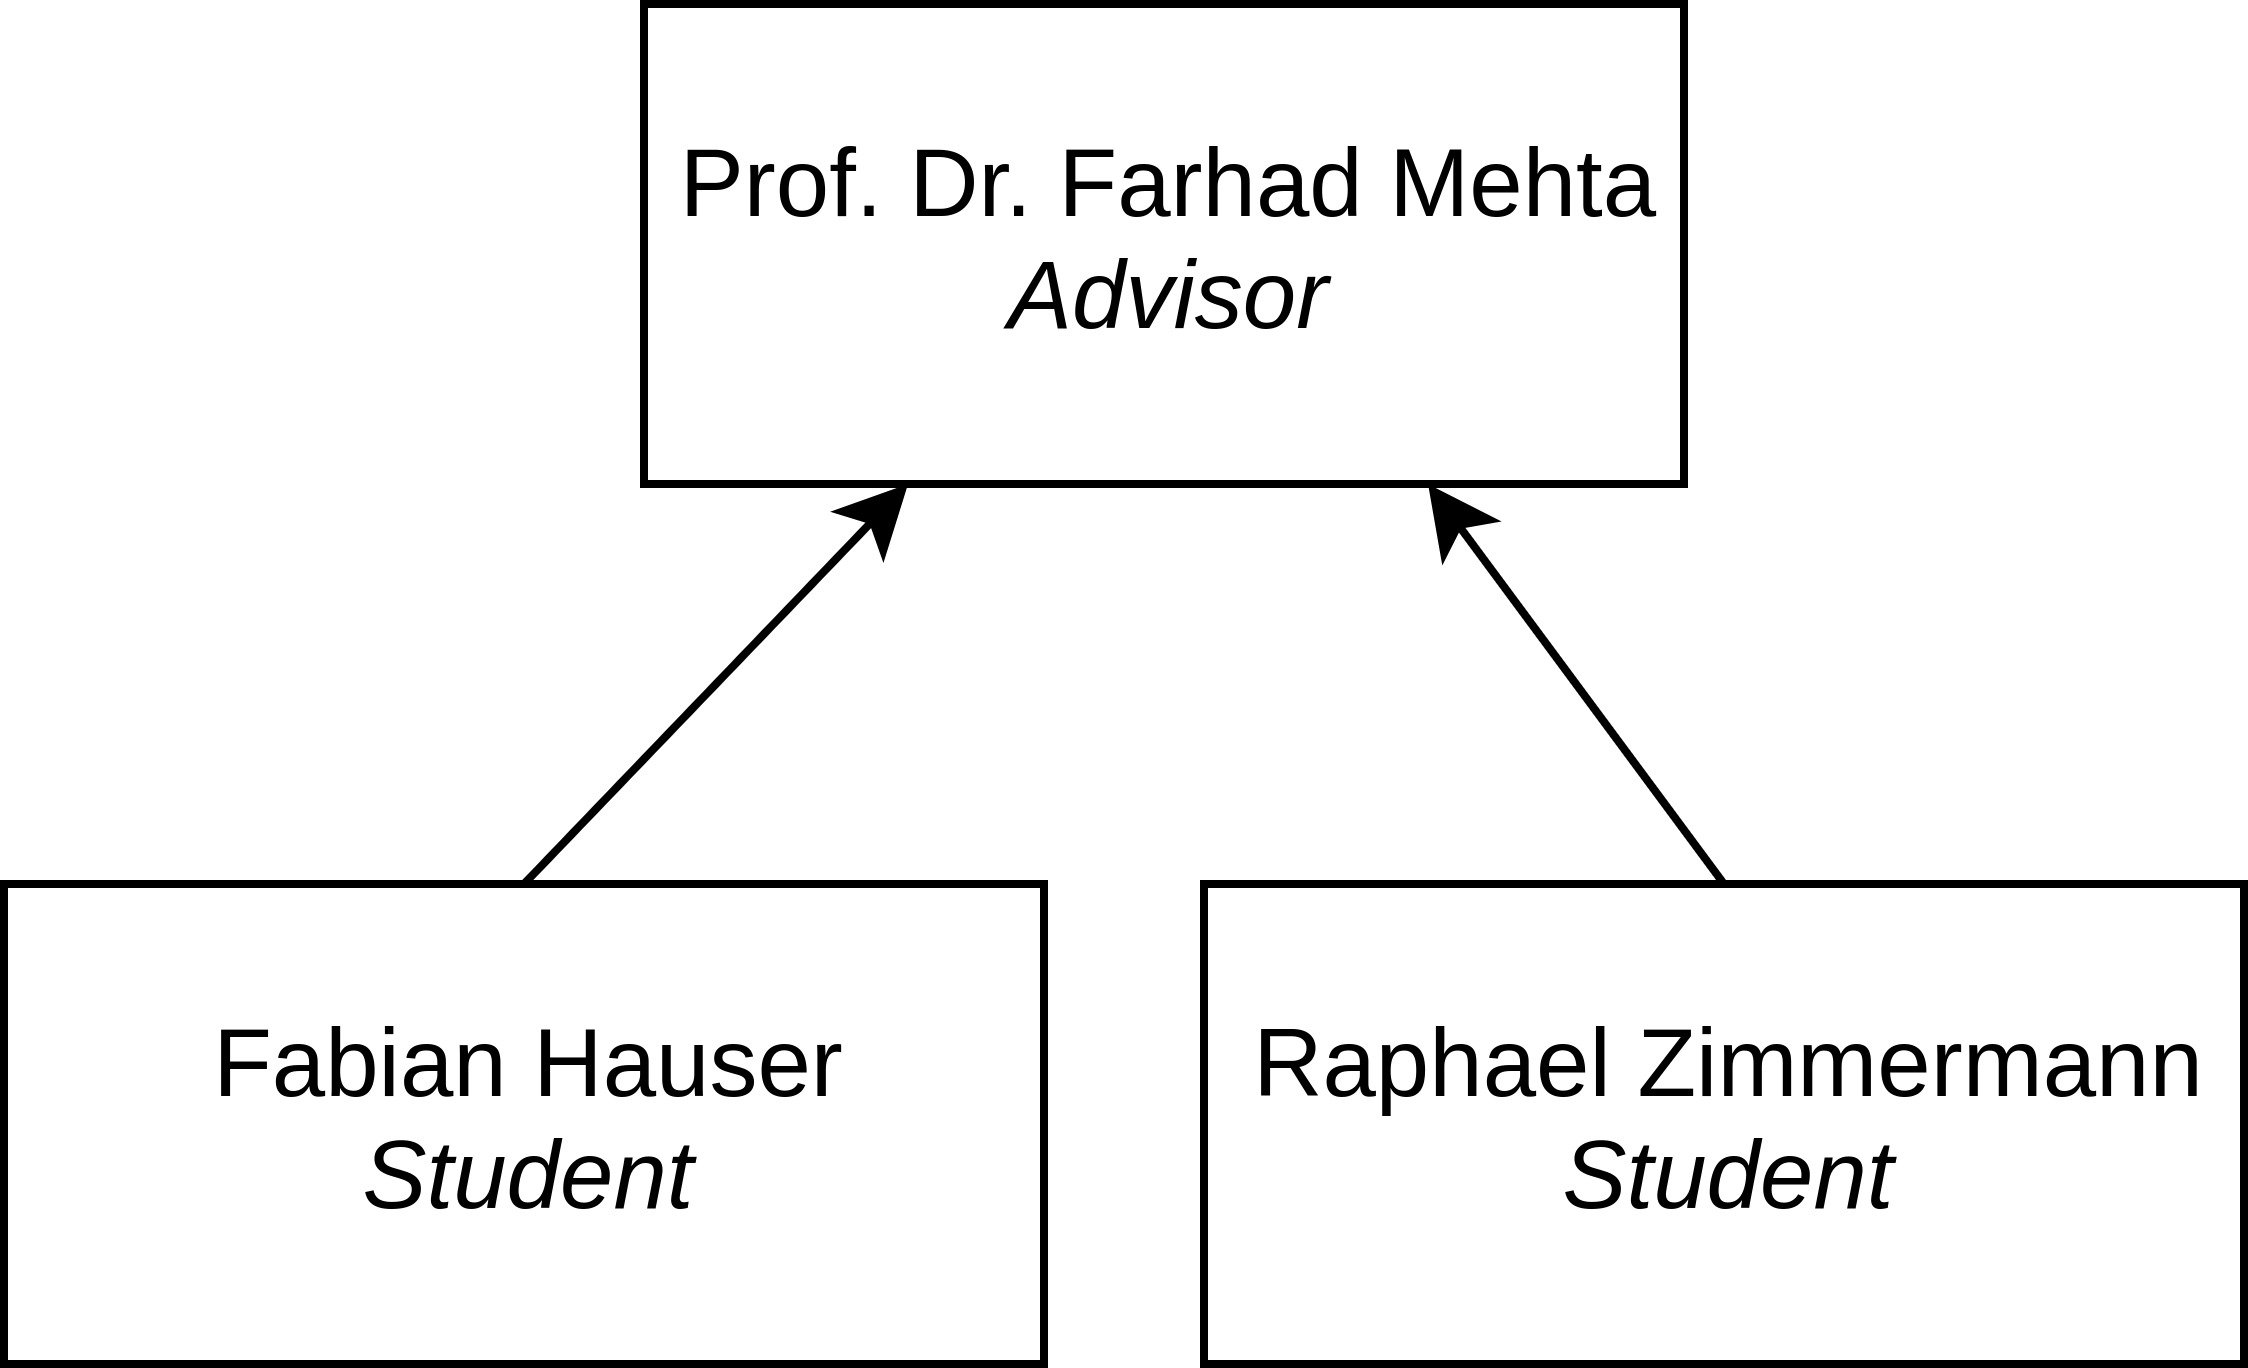
\includegraphics[width=0.5\linewidth]{resources/organigram}
	\caption[Organigram]{Project organization chart}
	\label{fig:organigram}
\end{figure}

\subsection{Roles}

Due to the small team size, most roles are performed by both team members.

\begin{description}
	\item[Raphael Zimmermann] project management, software engineering, quality assurance.
	\item[Fabian Hauser] infrastructure management, software engineering, quality assurance.
\end{description}

\section{Project Management}
\subsection{Components}

For a better overview and to allow us a sophisticated time assessment, we decided to group tasks into categories, i.e. JIRA components. Components represent processes, documents and products which are to be released.

Currently, tasks are separated into following components:

\begin{multicols}{2}
	\begin{itemize}
		\item Final Submission Document
		\item Concept Paper
		\item Management
		\item Poster
		\item Presentation
		\item Project Plan
		\item Prototype
	\end{itemize}
\end{multicols}

\subsection{Time Budget}

The project started with the Kickoff Meeting on 18.09.2017 and will be completed after 14 weeks by 22.12.2017.
The two team members are available for 240 hours each during this period which corresponds to a weekly time budget of 17.15 hour per person.

Apart from the statutory holidays, there are no further absences planned. Statutory holidays do not affect the weekly time budget.

\subsection{Schedule}
The project schedule is an iterative process based on elements of SCRUM. 

Due to the explorative nature of the project, we decided on a sprint duration of one week.
\subsubsection{Iterations \& Milestones}

\begin{figure}[h!]
	\centering
	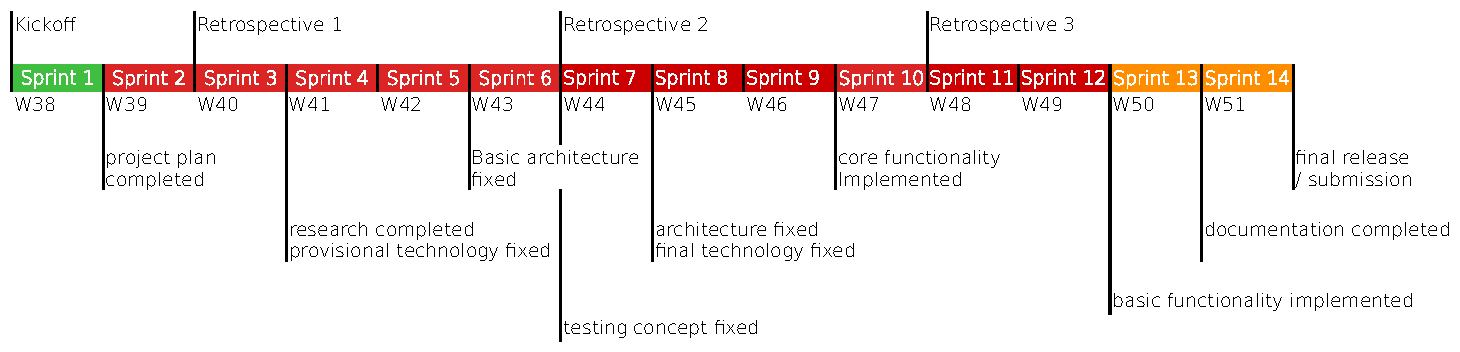
\includegraphics[width=1\linewidth]{resources/overview}
	\caption{Overview of the 14 iterations}
	\label{fig:overview}
\end{figure}

The goals and milestones resulting from each sprint are shown in Figure \ref{fig:sprint-details}.

\begin{figure}[h]
	\begin{sideways}
	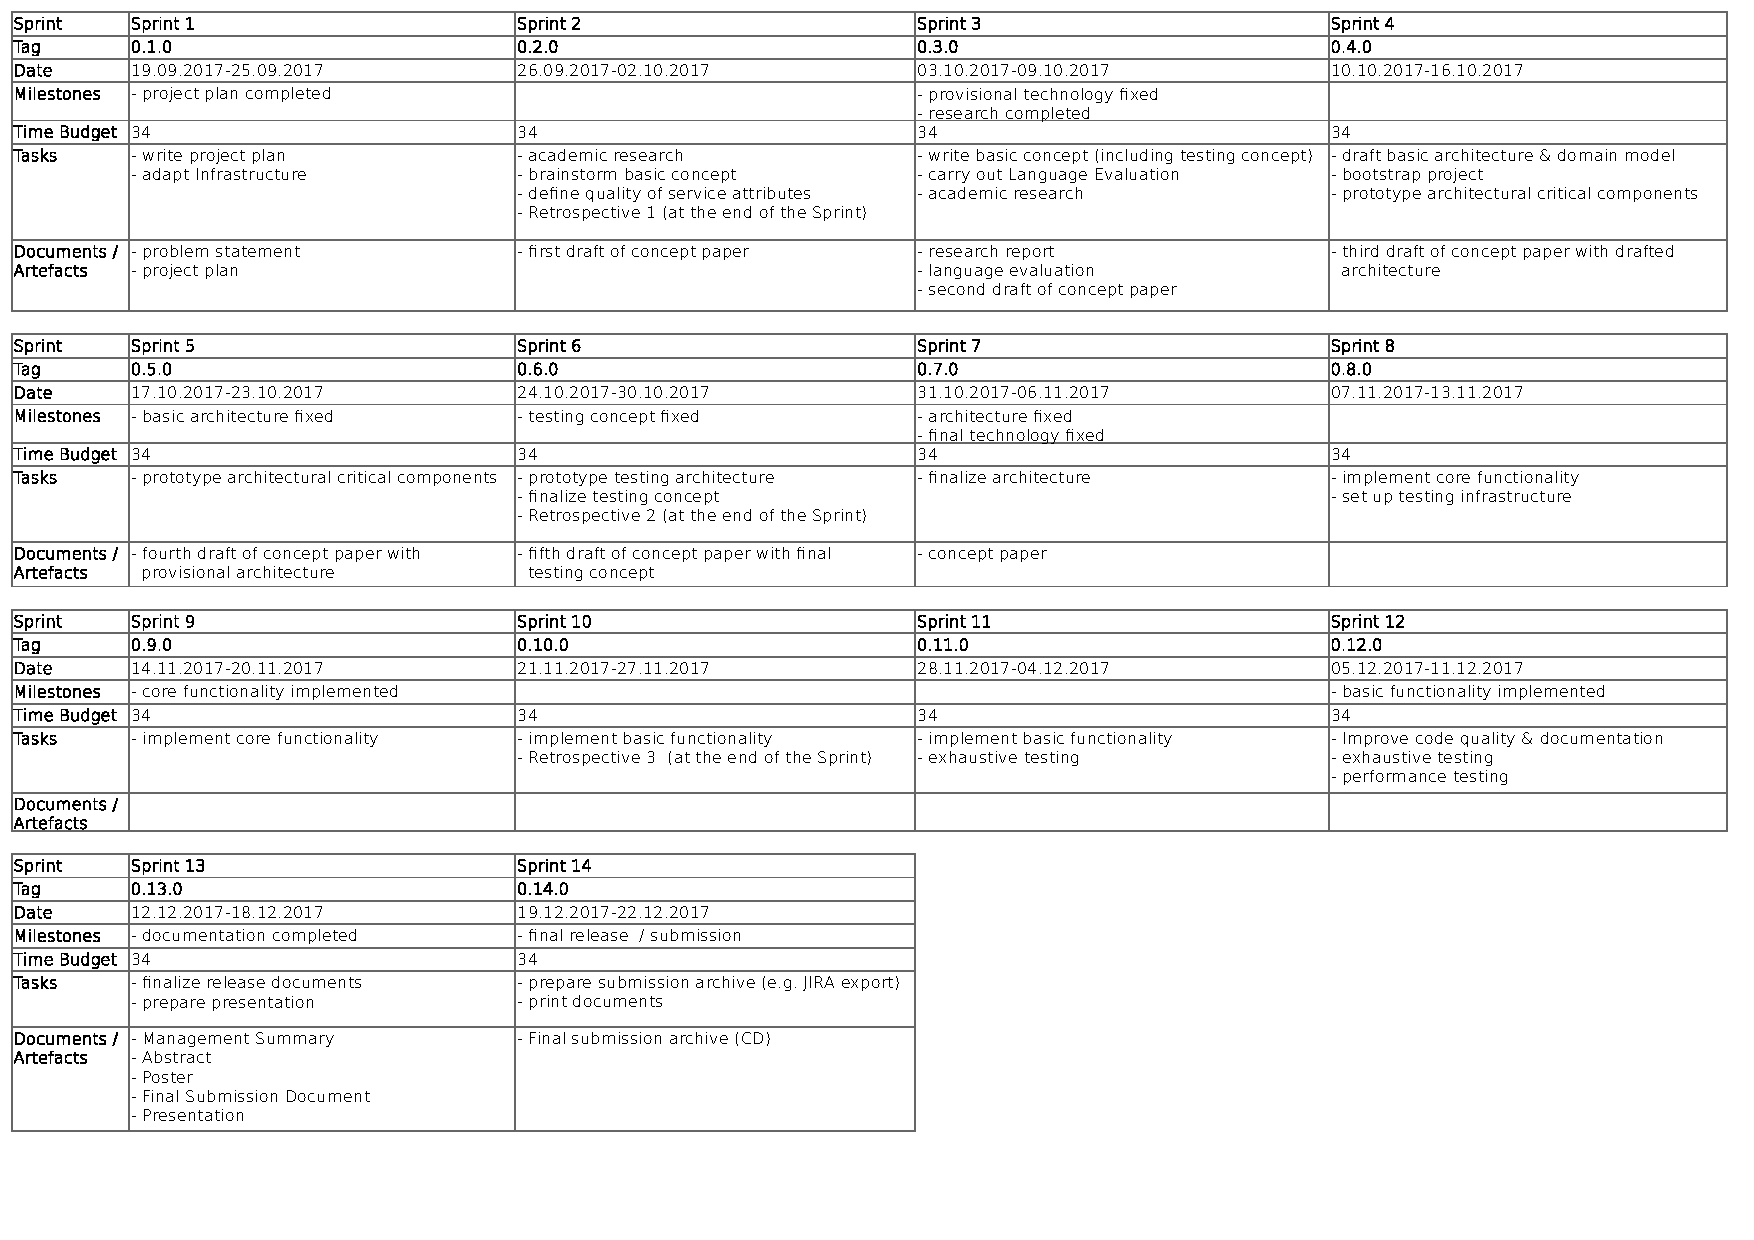
\includegraphics[scale=0.75]{resources/sprint_details}
	\end{sideways}
	\centering
	\caption{Detailed overview with tasks and milestones of all 14 sprints.}
	\label{fig:sprint-details}
\end{figure}


\subsubsection{Meetings}

The team works every Tuesday (10:00 - 17:00) together in the study project room and every Monday (08:00 - 17:00) remotely. Both days begin with a daily stand-up meeting taking no longer than 15 minutes. Sprint planning meetings are carried out on Tuesday at 10:00. Table \ref{meeting-time-budget} shows an overview of the total meeting time budget.

\begin{table}[]
	\centering
	\caption{Meeting Time Budget}
	\label{meeting-time-budget}
	\begin{tabular}{lll}
		\hline
		\textbf{Meeting Type}             & \textbf{Total Duration per Person} & \textbf{Total Duration for the Team} \\ \hline
		\textbf{Supervision Meetings}     & 14 hours                           & 28 hours                             \\
		\textbf{Standup Meetings}         & 7 hours                            & 14 hours                             \\
		\textbf{Sprint Planning Meetings} & 16 hours                           & 32 hours                             \\
		\textbf{Retrospective}            & 3 hours                            & 6 hours                              \\ \hline
		\textbf{Total}                    & 40 hours                           & 80 hours                            
	\end{tabular}
\end{table}

Regular meetings with the project advisor take usually place on Friday in Prof. Dr. Mehta's office. The agenda must be sent via email to all participants at least 24 hours prior the meeting.

Raphael Zimmermann will take meeting notes for every meeting. Meeting minutes are published on the project website afterwards.

\section{Risk Management}

An assessment of the project-specific risks is carried out in Table \ref{tbl:project-risks} as time loss during the whole project. The risk matrix in Table \ref{tbl:risk-matrix} provides an overview of the risk weighting.

To account for these risks, we reduce our weekly sprint time by the total weighted risk applicable to the planned task topics (on average approximately 20\%). We also review the risk assessment after every sprint, adapt it and take measures if necessary.


\begin{table}
	\centering
	\caption[Risk matrix]{The risk matrix. Numbers reference to the risk assessment Table \ref{tbl:project-risks}}
	\label{tbl:risk-matrix}
	\begin{tabu}{|l|c|c|c|}
		\hline
		\diagbox[width=9em,height=2.5em]{Probability}{Severity}
		  & High ($\geq 5d$) & Medium (2-5$d$) & Low ($\leq 2d$) \\ \hline
		High ($\geq 60\%$)
	      & 1 & & 6\\ \hline
		Medium (30-60\%)
		  & 8 & 2, 3 &  \\ \hline
		Low ($\leq 30\%$)
		  & & 4, 5, 7 & \\ \hline
	\end{tabu}
\end{table}


\begin{sidewaystable}
	\centering
	\caption[Risk assessment]{Risk assessment table. Time in hours over the total project duration.}
	\label{tbl:project-risks}
	\begin{tabu}{r l X X r r r}
		\hline
		\# & Title & Description & Prevention / Reaction & Risk [h] & Probability & = [h] \\ \hline

		1 & Problems with technology stack
		  & Parts of the selected technology stack are not well suited, incomplete or immature.
		  & Reflect the suitability of the chosen technology during the architecture draft.
		  & 60 & 60\% & 36\\

		2 & The architecture does not scale.
		  & The chosen architecture does not scale to the expected data volume or node size
		  & Invest an adequate amount of time in architecture design.
		  & 30 & 40\% & 12\\

		3 & Communication errors
		  & Errors due to miscommunication or misapprehension.
		  & Maintain a high level of interaction, precise specification of tasks responsibilities, conduct meetings if ambiguities exist.
		  & 20 & 50\% & 10\\

		4 & Problems with project infrastructure
		  & The used project infrastructure is not or only partially available, or data loss occurs within management software.
		  & Clean setup and self-hosting of the tools to prevent third-party dependencies.
		  & 30 & 30\% & 9 \\

		5 & Scope creep
		  & The project's scope is extended over the project course.
		  & Define the project scope and limitations precisely. Discuss changes with the project advisor.
		  & 30 & 30\% & 9\\

		6 & Missing architecture aspects
		  & The architecture-whitepaper does not fully cover all necessary aspects of the prototype.
		  & Invest an adequate amount of time in architecture design.
		  & 15 & 60\% & 9\\

		7 & Dependency errors
		  & There are errors/bugs in third-party dependencies, i.e. libraries.
		  & Carefully select libraries and limit thid-party dependency to a minimum.
		  & 20 & 30\% & 6\\

		8 & Missing dependency documentation
		  & Selected libraries are lacking proper documentation
		  & The documentation quality of a library should be a selection criterion.
		  & 15 & 40\% & 6\\

		 \hline
		& Total weighted risk & & & & & 97\\
		\hline
	\end{tabu}
\end{sidewaystable}


\section{Infrastructure}


\subsection{Project Management and Development}

For project management, document/code storage and continuous integration/deployment we utilise the corresponding products by Atlassian (JIRA, BitBucket, Bamboo, Crowd)\cite{atlassian-opensource}.

These applications are hosted on our HSR project server (\textit{sinv-56017.edu.hsr.ch}), which runs a standard Ubuntu Linux 17.04.


\subsubsection{Development Tools}

Since most development tools depend on the chosen technology and might change in the future, they are maintained separately on the project website \footnote{\url{https://www.redbackup.org/development/}}.

\subsection{Backup and Data Safety}

An incremental backup of the project server including the source code and documentation is created on an independent system (\textit{pin1262031.hsr.ch}) every night.

As our documents and code is stored in a git repository, they are also distributed on all development systems.


\section{Quality Measures}
To maintain a high standard of quality, we take the following measures:

\begin{multicols}{2}
	\begin{itemize}
	    \item short sprint reviews
	    \item three extended retrospectives
	    \item code reviews
	    \item automated unit and integration testing
	    \item publish all documentation on the project website using continuous integration/delivery.
	    \item using continuous integration for source code
	\end{itemize}
\end{multicols}

\subsection{Documentation}
The official documents such as the final submission document, the theoretical concept as well as this project plan are written in Latex and published on the project website \footnote{\url{https://www.redbackup.org}} as PDF documents. All other documents such as meeting minutes are written in Markdown and made available in HTML on the website as well.

The sources are in both cases kept under version control in the same repository, which allows us to use the same tools and processes for documentation and code. The continuous integration server builds and publishes the website whenever new changes are pushed to the repository.

\subsection{Project Management}
Because the project plan allows for an iterative process, we use JIRA with its SCRUM-Features (such as sprint creation or boards) for project management.

\subsubsection{Sprint Planning}
Each sprint is mapped to JIRA, which allows the project advisor to trace the project progress. Sprints are represented as boards on which the current state and assignee of any issue is easily visible ("To Do", "In Progress", "Review", "Done").


\subsubsection{Definition of Done}
An issue may be closed if \emph{all} of the following conditions are met:

\begin{itemize}
	\item All functionality conforms to the specification. Any deviations must be discussed and decided by the team.
	\item The source code is reasonably documented.
	\item No code is commented out.
	\item No warnings and errors by the compiler or any other quality tool.
	\item A review is performed and accepted in a pull request.
	\item The corresponding branch is merged into the stable branch (e.g. master).
	\item All documents are up to date including the project website.
	\item Reasonable unit and integration tests exist and pass.
	\item The complete continuous integration pipeline works.
	\item All time is logged.
\end{itemize}

\subsection{Development}

Since we are in a very early and agile stage we decided to use Github Flow\cite{github-flow}, a straightforward development workflow.

Since the effective technology will be fixed later in the project, concrete coding guidelines, tools, metrics and an error policy will be defined when appropriate.


\subsection{Testing}
All functionality must be automatically testable using continuous integration. Any non-trivial function/method must be verified with unit tests.

Integration tests verify extended test scenarios.

A minimal performance analysis will be carried out at the end of the project.

\bibliographystyle{abbrv}
\bibliography{refs}

\end{document}
